\section{Infographic Posters}

Infographic posters are a creative way to turn complex data into simple, engaging visuals. By using graphics, key facts, and clear messages, they help people quickly understand important information. Whether for students, professionals, or the general public, these posters make it easier to connect with the audience, spark interest, and improve understanding and memory.

\subsection*{Why Use Infographic Posters?}

\begin{itemize}
    \item \textbf{Make Complex Things Simple:} Infographics turn big numbers or difficult ideas into clear and easy visuals that anyone can understand.
    
    \item \textbf{Grab Attention Quickly:} Bright colors, icons, and charts make people stop and look much more than plain text or long tables.
    
    \item \textbf{Tell a Clear Story:} With a good layout, infographics guide the reader through the key message step by step, making your point easy to remember.
    
    \item \textbf{Reach More People:} Infographics are perfect for sharing on social media, in reports, classrooms, and community meetings.
    
    \item \textbf{Save Time for the Reader:} People don’t always have time to read long reports. A quick glance at a poster can give them the main idea in seconds.
    
    \item \textbf{Good for All Ages:} From students to professionals, everyone can benefit from a well-made visual. It breaks language barriers and keeps learning fun.
\end{itemize}


\subsection*{Key Components of an Effective Infographic Poster}

\begin{itemize}
    \item \textbf{Clear Title and Short Intro:} Start with a catchy title and a quick sentence to explain what your poster is about. This helps people know right away why they should care.

    \item \textbf{Easy-to-Follow Layout:} Arrange your content in a logical order like top to bottom or left to right so the viewer’s eyes naturally move through the story.

    \item \textbf{Visuals That Speak:} Use simple charts, graphs, icons, or maps to show your message. A good visual can say more than a whole paragraph.

    \item \textbf{Less Text, More Meaning:} Keep sentences short and to the point. Use plain language so that even someone with no background knowledge can understand it.

    \item \textbf{Clean and Consistent Design:} Stick to a small set of colors and fonts to keep the poster neat and easy to read. Avoid clutter.

    \item \textbf{Source and Credits:} Always include where your data comes from and who helped you. It shows honesty and builds trust.

    \item \textbf{Audience-Friendly Language:} Use words and examples that fit your audience whether they’re students, farmers, teachers, or policy-makers.

    \item \textbf{Use of Space Wisely:} Make sure there’s enough empty space (white space) so the poster doesn’t feel crowded. This makes it easier on the eyes.

\end{itemize}


\subsection*{Creating an Infographic Poster Using Canva}

Canva is an easy-to-use online tool that helps you create beautiful visuals without needing any graphic design experience. It’s perfect for making infographic posters, presentations, social media posts, and more. With thousands of free templates and drag-and-drop features, Canva makes design feel simple and fun. Whether you're a student, teacher, or researcher, you can turn your ideas and data into eye-catching visuals in just a few clicks. All you need is an internet connection and a bit of creativity!\\
Here is a simple step-by-step guide to get started:

\begin{enumerate}
    \item \textbf{Sign Up and Log In:} Visit \url{https://www.canva.com} and create a free account or log in.
    \item \textbf{Select a Template:} Use the search bar to find ``Infographic'' templates. Choose one that matches your theme or style.
    \item \textbf{Customize Layout and Design:} Replace placeholder text with your own headings, descriptions, and data insights. Adjust font sizes, colors, and styles to suit your branding or preference.
    \item \textbf{Add Visual Elements:} Upload your charts or graphs as images, or use Canva’s built-in icons, shapes, and illustrations to enhance your story.
    \item \textbf{Incorporate Data Visualizations:} If you have data charts (from R, Excel, etc.), export them as images and upload them to Canva to place in your design.
    \item \textbf{Review and Edit:} Check for clarity, consistency, and visual appeal. Make sure your narrative flows well and key points stand out.
    \item \textbf{Download and Share:} Download your infographic as a PDF, PNG, or JPEG. You can print it, embed it in presentations, or share it online.
\end{enumerate}

\subsection*{Tips for Effective Infographics}

\begin{itemize}
    \item Keep it simple — avoid clutter.
    \item Use contrasting colors to highlight important information.
    \item Limit fonts to two or three types for consistency.
    \item Use whitespace effectively to separate sections.
    \item Tell a story — every element should support the main message.
\end{itemize}

By leveraging tools like Canva, you can create impactful infographic posters that communicate your data stories clearly and professionally, engaging a wide audience with minimal effort.

\begin{figure}[h]
\centering
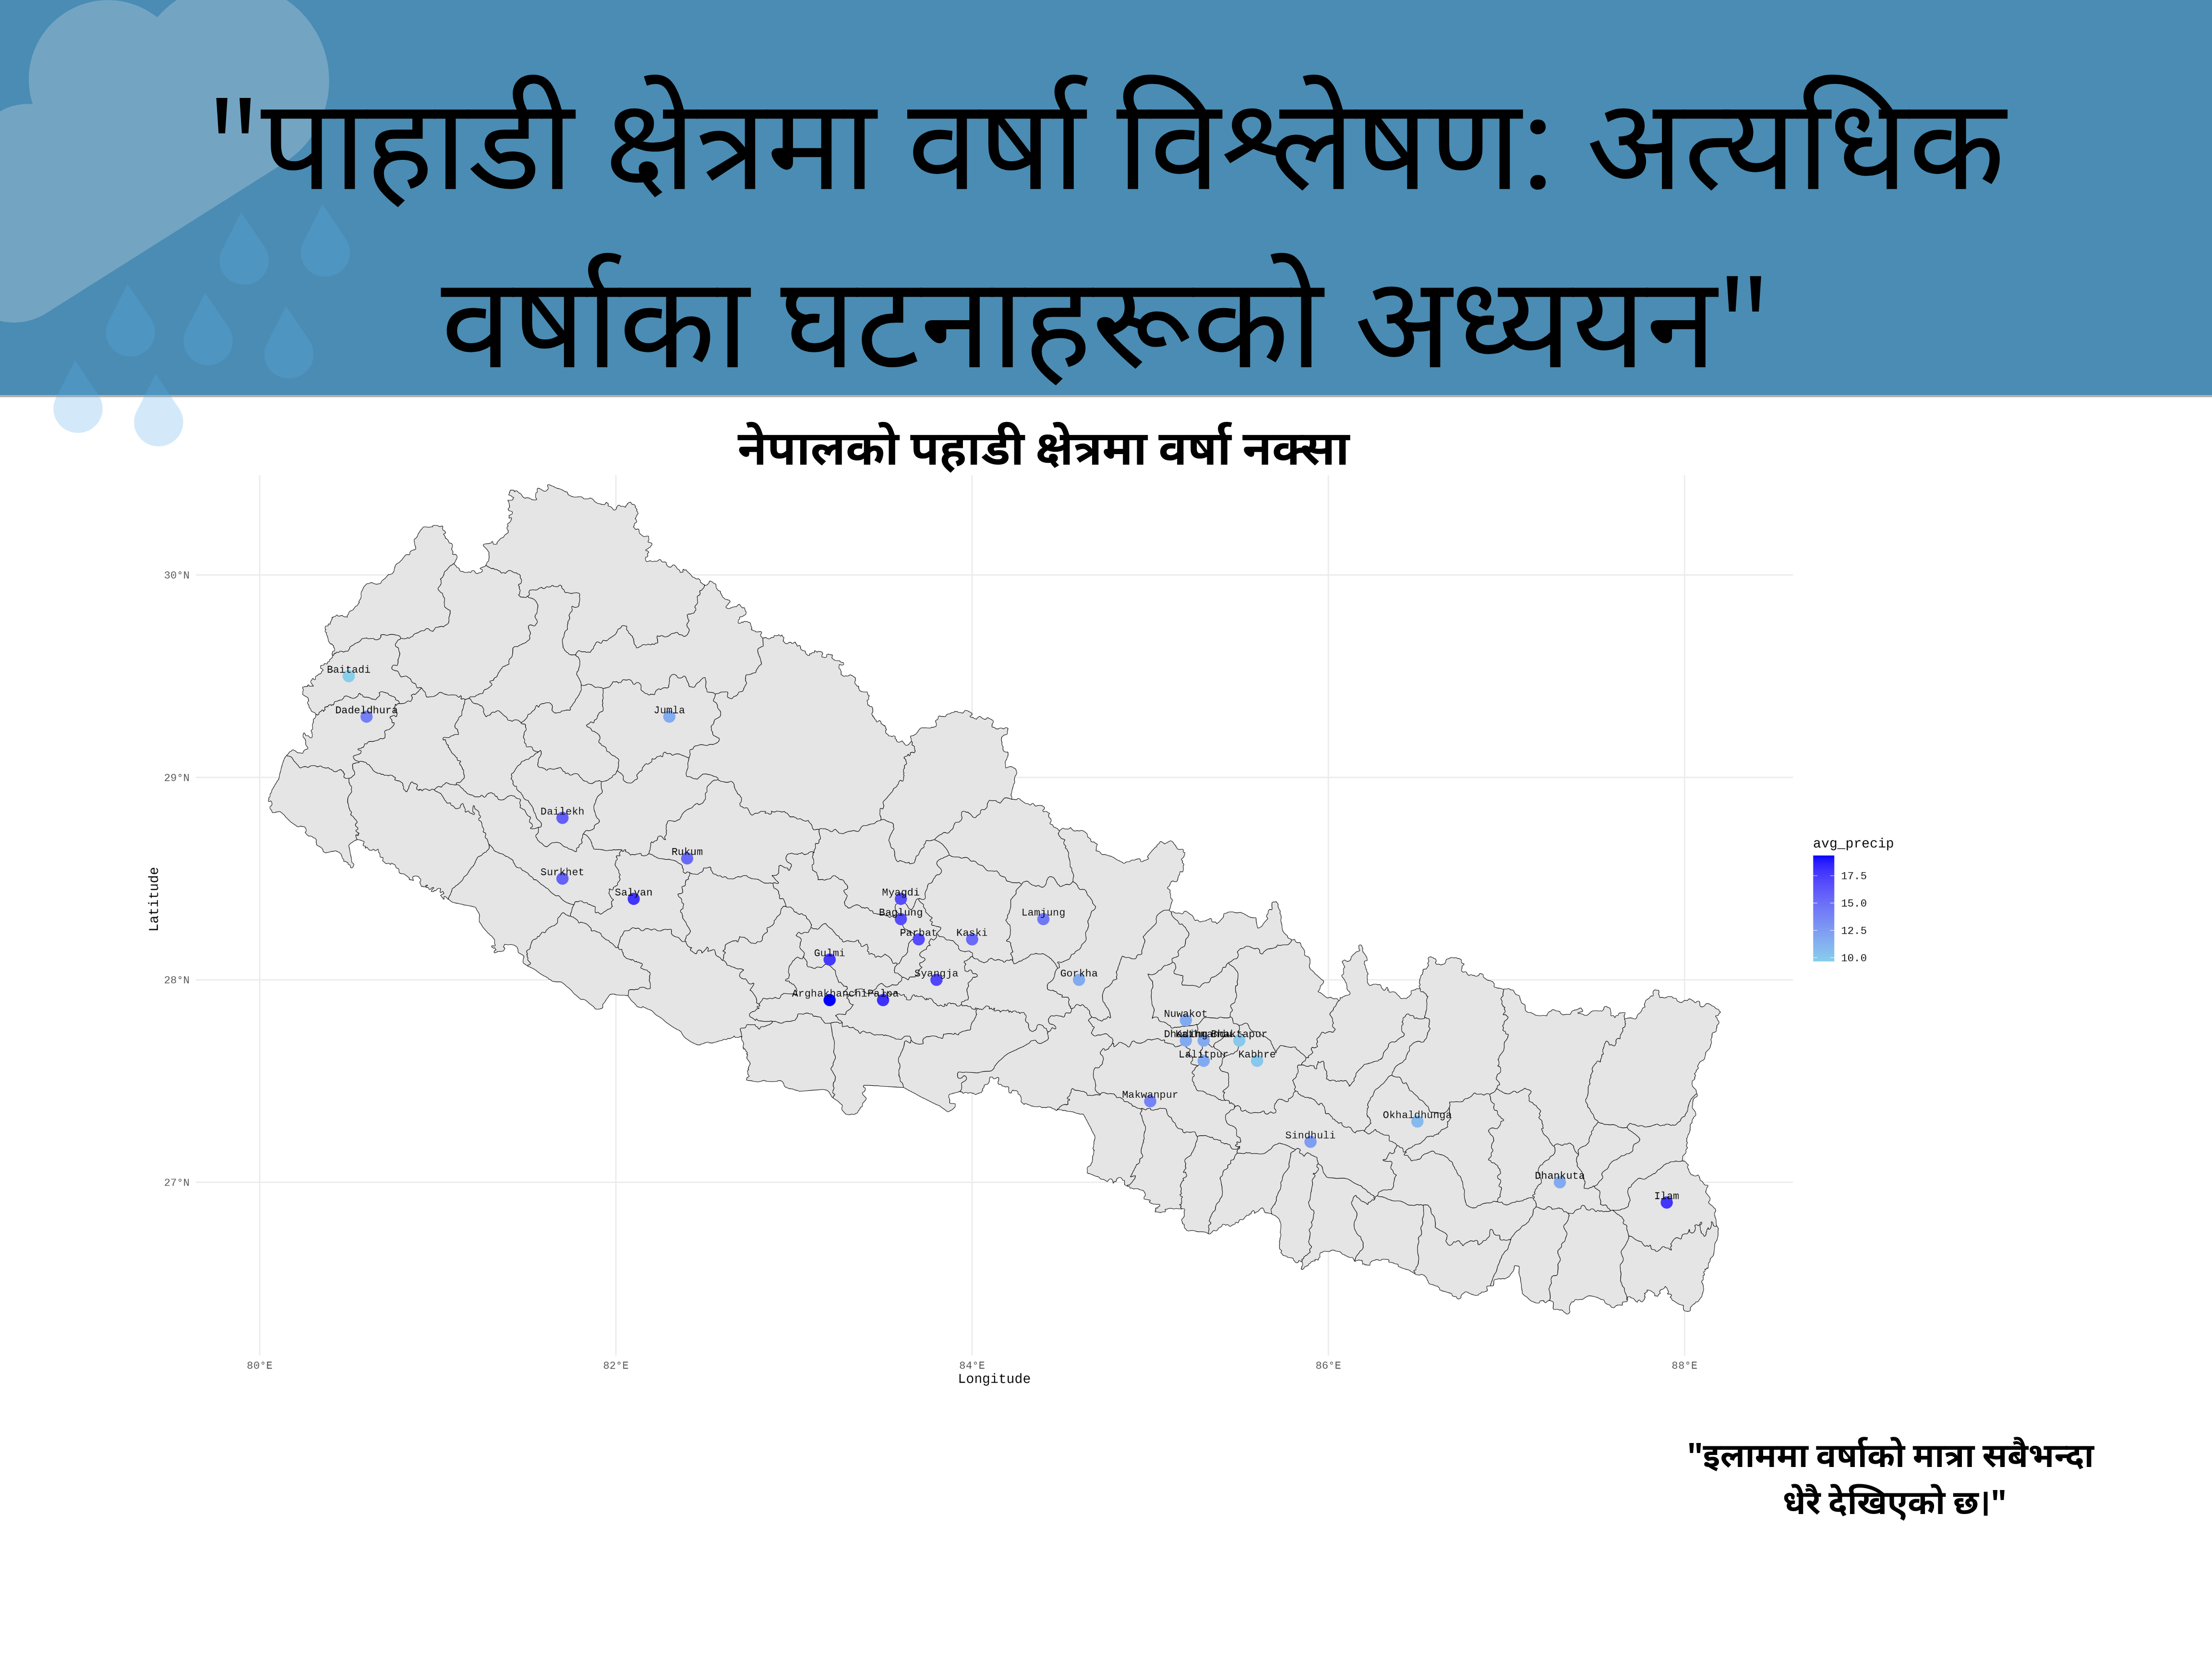
\includegraphics[width=0.7\textwidth]{figures/info1.png}
\end{figure}

\begin{figure}[h]
\centering
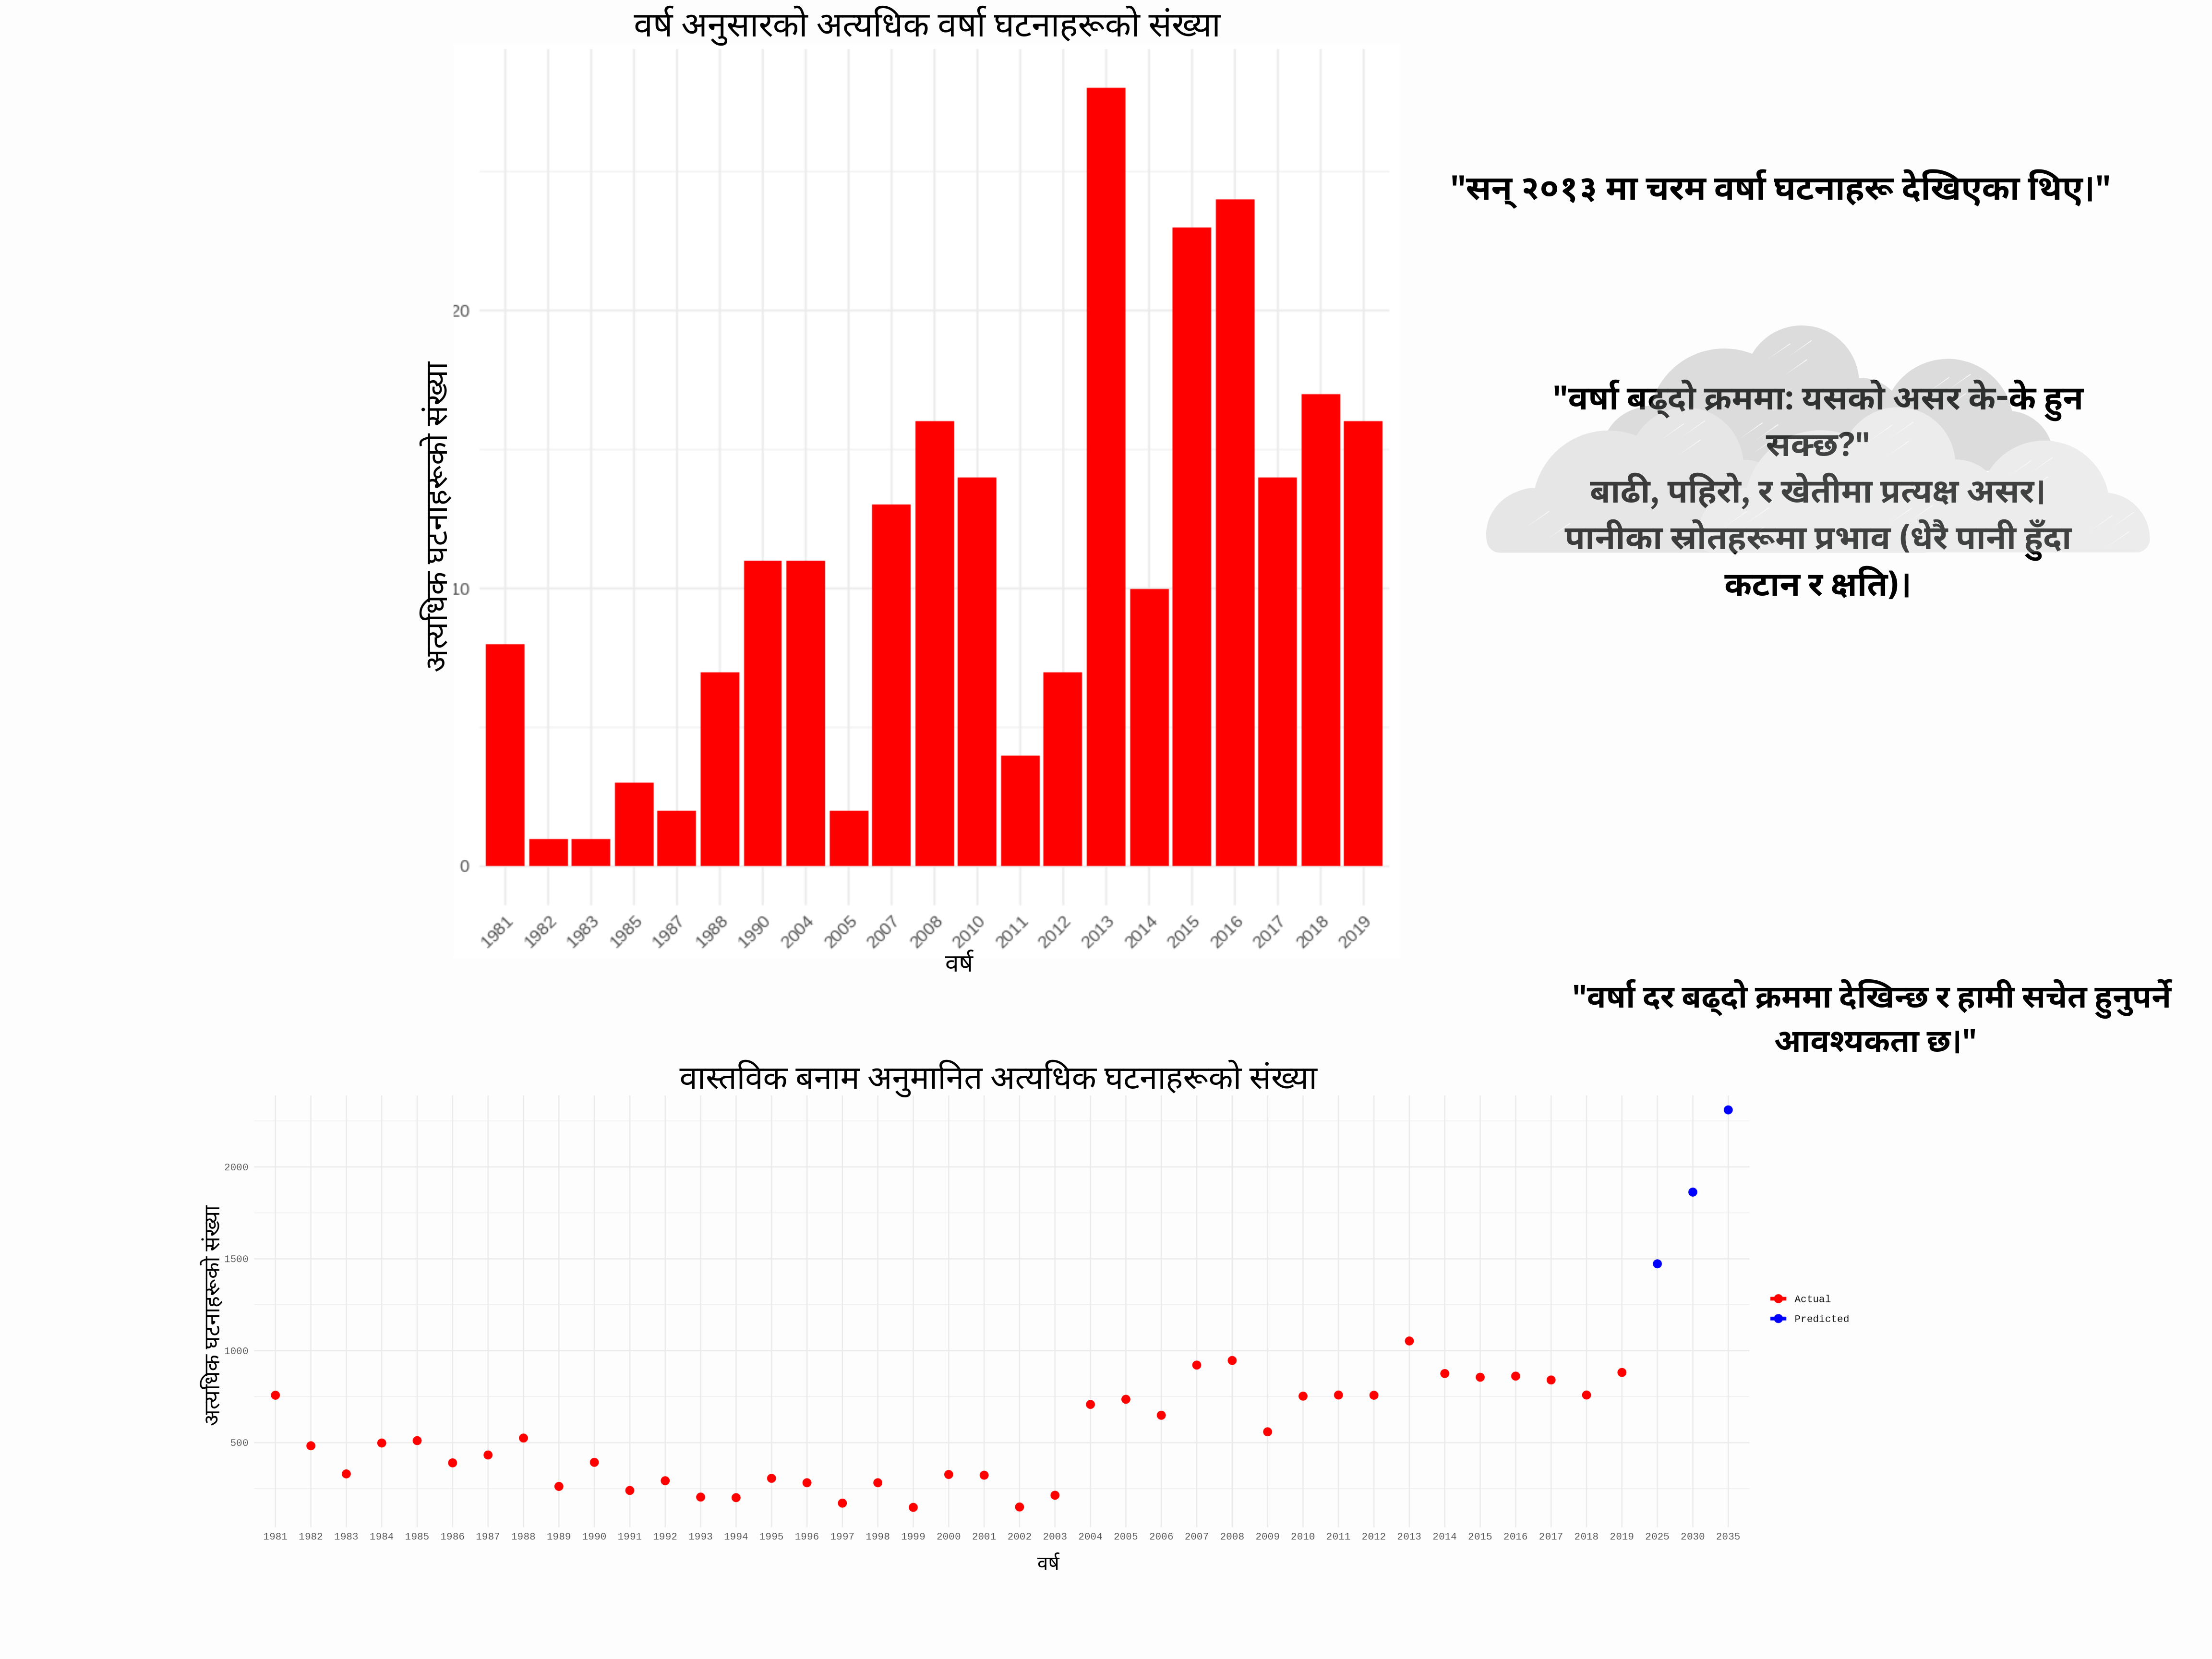
\includegraphics[width=0.7\textwidth]{figures/info2.png}
\caption{Figure 7.1: Infographic Poster}
\end{figure}

\clearpage